
\chapter{Doing design (2 of 2)}
\label{design2}

\section{The two domains}

Before we dive back in and complete our two examples from last chapter, let me
make an observation about the classes in an OO program. They tend to come from
two different sources. We call these two categories ``the \textbf{problem
domain}'' and ``the \textbf{solution domain}.''

\index{problem domain}
The problem domain provides classes that relate to the \textit{problem} the
program is designed to solve. A key give-away of a problem domain class is
that the user herself recognizes the term used. She thinks of that entity as
central in what the system does/is.

\index{bid@\texttt{Bid}}
\index{auction@\texttt{Auction}}
\index{item@\texttt{Item}}
\index{seller@\texttt{Seller}}
\index{buyer@\texttt{Buyer}}
\index{eBay}
For instance, in an eBay type application, classes like \texttt{Bid},
\texttt{Auction}, \texttt{Item}, \texttt{Seller}, and \texttt{Buyer} are all
from the problem domain. eBay users think about, and talk about, these very
concepts when they think about the system, even if ``code'' never crosses their
mind.

\index{solution domain}
\index{smtpServer@\texttt{SMTPServer}}
\index{messageListener@\texttt{MessageListener}}
\index{loginPane@\texttt{LoginPane}}
The other source of classes is the solution domain, which consists of
supportive classes that don't really represent things about the problem
itself, but which are necessary to solve the problem. Suppose an email
application had a \texttt{SMTPServer} class. This would represent a connection
to a piece of hardware that acted as a SMTP (Simple Mail Transfer Protocol)
server to deliver electronic mail. Is this class's functionality necessary to
send email, as the email application needs to do? Yes. But does an everyday
email user think about ``SMTP Servers'' being involved? Likely not. The same
could be said of classes like ``\texttt{DatabaseConnection},''
``\texttt{MessageListener},'' and ``\texttt{LoginPane}.''  These classes all
perform critical supporting functions and therefore are vital to the operation
of the system. At the same time, though, we recognize that they are tangential
to the main purpose of the system as the user sees it: users of Wikipedia
don't think in terms of ``database connections,'' nor email users of ``message
listeners,'' nor Spotify users of the ``login panes'' in their UI. So we
relegate those classes to a different realm of sorts; one that contains
classes to perform functions, not to represent the domain's reality.

\index{connection}
\index{Spotify}
\index{song@\texttt{Song}}
\index{playlist@\texttt{Playlist}}
You might wonder which of the two domains is most important to get right. The
answer is unquestionably the \textit{problem domain}. Think about it: if
Spotify decided to change their underlying storage mechanism, and therefore
needed to retire their \texttt{DatabaseConnection} class, that's not a big deal to their
user base. If the new program version is implemented well and doesn't
introduce a lot of lagginess or bugs, the user will be unaware that it was
even changed. But change something in the \textit{problem} domain, and whoo
Nellie, the whole system experiences a change. Imagine if Spotify got rid of
their \texttt{Song} or \texttt{Playlist} classes. The entire application would
have to perform differently, with serious consequences for the user.


\section{Turning CRC cards into UML}

\index{CRC card}
When we last left our heroes in chapter~\ref{design1}, they had succeeded in
turning an English language description into a set of CRC cards. That's a ton
of progress. All they need to do now is complete the trick: turn those CRC
cards into a UML class diagram, and then into Java code. And that's just what
we'll do in the rest of this chapter.

\subsection{The bike store example, continued}

\index{CRC card}
Reacquaint yourself with the CRC cards on
pp.~\pageref{bikeCRC1}--\pageref{bikeCRC2}. These reflect some of the candidate
classes from our bike store example.

You've probably already figured out that when turning a CRC card into a class,
the ``Knows:'' section typically gets turned into instance variables, and the
``Can:'' section becomes methods. It isn't always a straightforward one-to-one
mapping, but it's often pretty close.

Let's start with \texttt{Shipment} on p.~\pageref{bikeCRC1}. The four items on
its ``knows'' items all call out for instance variables:

\begin{samepage}
\begin{compactitem}
\item ``which vendor is delivering it'': type \texttt{Supplier}
\item ``which purchase order it is fulfilling'': type
\texttt{ArrayList<PurchaseOrder>}
\item ``the expected arrival date'': type \texttt{Date}\footnote{The
\texttt{java.util} package has a \texttt{Date} class that represents all the
necessary aspects of a day in time on planet Earth. This is a better choice
than a \texttt{String} or a handful of \texttt{int}s to do it ourselves.}
\item ``the items in each shipment'': type \texttt{ArrayList<Item>}
\end{compactitem}
\end{samepage}

\index{instance variable (inst var)}
\index{association}
In terms of a UML diagram, we would depict the third of these as an entry in
the middle class box (see Figure~\ref{fig:bikeClassDiag}), and the other three
as associations to other classes. Also, the ``can'' list mentions that we can
update the ``status'' of a \texttt{Shipment}, which will probably entail a
\texttt{String status} inst var as well.

As for its methods, we have getters and setters for status and supplier, and
also the ability to \texttt{.cancel()} and \texttt{.receive()} the shipment. At
this point we're sort of guessing as to argument types and return values for
each method; it seems to me that both \texttt{.cancel()} and
\texttt{.receive()} can simply be argument-less and return \texttt{void}. (We'll
amend this assumption later if it turns out to be incorrect.) The finished
class is in the upper-left corner of Figure~\ref{fig:bikeClassDiag}.

\begin{figure}[ht]
\centering
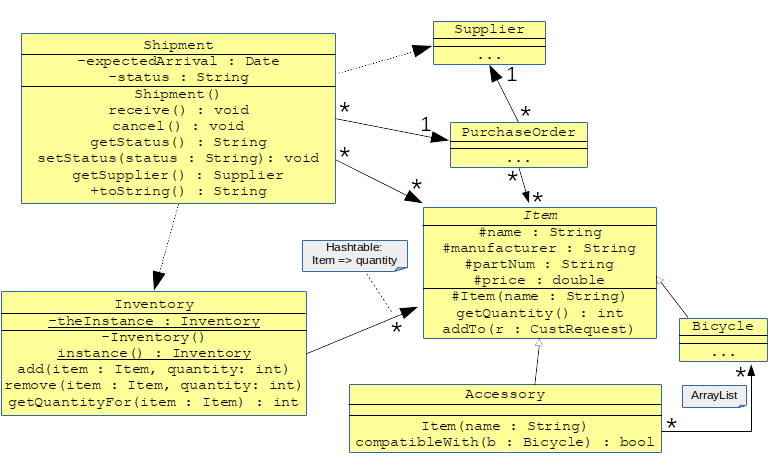
\includegraphics[width=.95\textwidth]{bikeClassDiag.png}
\caption{A first crack at converting CRC cards from Chapter~\ref{design1}'s
bicycle example into UML.}
\label{fig:bikeClassDiag}
\end{figure}

We didn't actually write full CRC cards for all the classes in this design, but
that's okay: to complete \texttt{Shipment}, we can just sketch in temporary
placeholders for classes like \texttt{PurchaseOrder} and \texttt{Supplier}.

The \texttt{Accessory} card from p.~\pageref{bikeCRC2} has a number of
``knows'' entries, though when we consider where to put them, we realize that
many of them will go in the abstract \texttt{Item} class. Only an
\texttt{ArrayList} of \texttt{Bicycle} objects seems appropriate as an inst var
for the \texttt{Accessory} subclass specifically, and that is what the diagram
shows. Since p.~\pageref{bikeCRC2} tells us that an \texttt{Accessory} ``knows
its compatible bicycle models,'' it seems appropriate for the class to support
a \texttt{.compatibleWith()} method that returns a \texttt{boolean} indicating
whether the accessory in question is compatible with a particular bike.

\index{singleton}
Finally, our \texttt{Inventory} CRC card (also on p.~\pageref{bikeCRC2}) tells
us that in addition to the standard Singleton stuff, we need to be able to
\texttt{.add()} and \texttt{.remove()} quantities of items from the
\texttt{Inventory}, as well as get a current count of how many units of an
\texttt{Item} we have in stock. One way to implement this would be through a
\texttt{Hashtable} that maps each \texttt{Item} to an in-stock quantity, and
that is what Figure~\ref{fig:bikeClassDiag} shows.

I think you'll agree this is a pretty straightforward, though not completely
mechanical, process. CRC cards have already identified the lion's share of the
program's important static structure, and go a long way towards giving us a UML
class diagram from which we can write code.

\subsection{The Uno! game example, continued}

\textit{...Stephen completes this in summer 2019...}

% "god classes"
% TODO: Goals:
% \begin{itemize}
% \itemsep.1em
% \item Each class does one thing well.
% \item Distributed responsibility (no god classes, \textit{e.g.}).
% \item Encapsulation (each class's design decisions are insulated from others).
% \end{itemize}

